% 按固定来源第3扫描页四个候选图重绘；保留 x=1 参考线、y=1 虚线及折线相对关系。
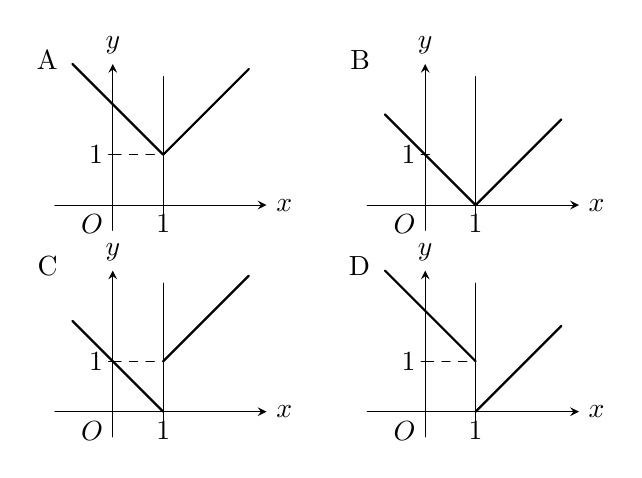
\begin{tikzpicture}[x=0.64cm,y=0.64cm,line cap=round,line join=round,>=stealth]
\begin{scope}
  \draw[->] (-1.15,0)--(3.05,0) node[right] {$x$};
  \draw[->] (0,-0.5)--(0,2.8) node[above] {$y$};
  \draw[thin] (1,-0.35)--(1,2.55);
  \draw[thick] (-0.8,2.8)--(1,1)--(2.7,2.7);
  \draw[dashed] (0,1)--(1,1);
  \draw[thin] (-0.08,1)--(0.08,1) (1,-0.08)--(1,0.08);
  \node[below left] at (0,0) {$O$};
  \node[left] at (0,1) {$1$};
  \node[below] at (1,0) {$1$};
  \node[above left] at (-0.9,2.5) {A};
\end{scope}
\begin{scope}[shift={(6.2,0)}]
  \draw[->] (-1.15,0)--(3.05,0) node[right] {$x$};
  \draw[->] (0,-0.5)--(0,2.8) node[above] {$y$};
  \draw[thin] (1,-0.35)--(1,2.55);
  \draw[thick] (-0.8,1.8)--(1,0)--(2.7,1.7);
  \draw[thin] (-0.08,1)--(0.08,1) (1,-0.08)--(1,0.08);
  \node[below left] at (0,0) {$O$};
  \node[left] at (0,1) {$1$};
  \node[below] at (1,0) {$1$};
  \node[above left] at (-0.9,2.5) {B};
\end{scope}
\begin{scope}[shift={(0,-4.1)}]
  \draw[->] (-1.15,0)--(3.05,0) node[right] {$x$};
  \draw[->] (0,-0.5)--(0,2.8) node[above] {$y$};
  \draw[thin] (1,-0.35)--(1,2.55);
  \draw[thick] (-0.8,1.8)--(1,0);
  \draw[thick] (1,1)--(2.7,2.7);
  \draw[dashed] (0,1)--(1,1);
  \draw[thin] (-0.08,1)--(0.08,1) (1,-0.08)--(1,0.08);
  \node[below left] at (0,0) {$O$};
  \node[left] at (0,1) {$1$};
  \node[below] at (1,0) {$1$};
  \node[above left] at (-0.9,2.5) {C};
\end{scope}
\begin{scope}[shift={(6.2,-4.1)}]
  \draw[->] (-1.15,0)--(3.05,0) node[right] {$x$};
  \draw[->] (0,-0.5)--(0,2.8) node[above] {$y$};
  \draw[thin] (1,-0.35)--(1,2.55);
  \draw[thick] (-0.8,2.8)--(1,1);
  \draw[thick] (1,0)--(2.7,1.7);
  \draw[dashed] (0,1)--(1,1);
  \draw[thin] (-0.08,1)--(0.08,1) (1,-0.08)--(1,0.08);
  \node[below left] at (0,0) {$O$};
  \node[left] at (0,1) {$1$};
  \node[below] at (1,0) {$1$};
  \node[above left] at (-0.9,2.5) {D};
\end{scope}
\end{tikzpicture}
